\chapter{Part II: Gray-Scott Systems} \label{gray-scott}

To learn Gray-Scott models, we extend our evolutionary algorithm toolkit further to include more diverse methods such as evolutionary strategies and particle swarm optimization.

\section{Learning Process}

\subsection{Simulator} \label{subsec:simulator}

In this setting, we run a discretized simulation of a continuous system so there are more subtleties to consider. We use two NumPy arrays of floats to store the density of $u$ and $v$ across the CA. To simulate the change in these densities efficiently, we use a pair of finite-difference equations that approximate the continuous partial differential equations in Def~\ref{def:reaction-diffusion}. We first define discrete approximations for the derivative of each density.
\begin{definition}[Gray-Scott Model]\label{def:gs}
\begin{align*}
  \dot{u} &= -uv^2 + f(1-u) + r_u \mathcal{D}(u)\\
  \dot{v} &= uv^2 - (f+k)v + r_v \mathcal{D}(v)
\end{align*}
\end{definition}
Each equation has 3 terms. From left to right, these are the reaction term, the external term and the diffusion term. This is exactly the same as the continuous definition with the exception of the discrete Laplace operator $\mathcal{D}$ which replaces the continuous Laplacian $\Delta$. Calculating the first two terms is simple enough as we are given the feed and kill rates.  However, the third term must approximate the Laplacian which is usually computationally intensive to calculate. To do this, we use a kernel that, when convolved over the density matrices of $u$ and $v$, produces matrices whose entries are approximations of $\Delta u(x,y)$ and $\Delta v(x,y)$ respectively. Different kernels have been used for this convolution in the literature. One example used by in Compeau's Biological Modelling book\cite{compeau} is
\[
  K= \begin{bmatrix}
    0.05 & 0.2 & 0.05\\
    0.2 & -1 & 0.2\\
    0.05 & 0.2 & 0.05
  \end{bmatrix}
\]
Another popular choice is the nine-point stencil\cite{rosser1975nine}.
\[
  \Delta^{(9)}_h = \begin{bmatrix}
    0.25 & 0.5 & 0.25\\
    0.5 & -3 & 0.5\\
    0.25 & 0.5 & 0.25
  \end{bmatrix}
\]
Testing on a few examples revealed that both kernels capture complex diffusion behaviour with similar effectiveness. However, the choice of kernel is not arbitrary and these two choices are well principled. We briefly outline the reasoning behind the nine-point stencil. If we briefly consider $u$ as a function of only $x$ (i.e fix $y$ and $t$ constant) and rearrange the Taylor series expansions for $u(x+h)$ and $u(x-h)$, we get
\begin{align*}
  \pdv{u}{x} &= \frac{u(x+h) - u(x)}{h} - \frac{u^{(2)}(x)}{2!}h - \frac{u^{(3)}(x)}{3!}h^2 - \frac{u^{(4)}(x)}{4!}h^3 - ... \\
  \pdv{u}{x} &= - \frac{u(x-h) - u(x)}{h} + \frac{u^{(2)}(x)}{2!}h - \frac{u^{(3)}(x)}{3!}h^2 + \frac{u^{(4)}(x)}{4!}h^3 - ...
\end{align*}
Subtracting one from the other yields the 3-point stencil approximation for the Laplacian in one dimension denoted $\Delta^{(3)}u(x)$.
\begin{align*}
  0 &= \frac{u(x+h) + u(x-h) - 2u(x)}{h} - u^{(2)}(x)h - 2\frac{u^{(4)}(x)}{4!}h^3 + ...\\
  \implies \pdv{u}{x^2} &=  \underbrace{\frac{u(x-h) -2u(x) + u(x+h)}{h^2}}_{\let\scriptstyle\textstyle
  \substack{=: \Delta^{(3)}u(x)}} + O(h^2)
\end{align*}
By combining two of these we get a two dimensional 5-point stencil.
\begin{align*}
  \Delta u(x, y) &= \pdv{u}{x^2} + \pdv{u}{y^2}\\
                     &\approx \frac{u(x-h, y) -2u(x, y) + u(x+h, y)}{h^2} + \frac{u(x, y-h) -2u(x, y) + u(x, y+h)}{h^2}\\
                     &= \frac{u(x-h, y)+ u(x+h, y) -4u(x, y) + u(x, y-h) + u(x, y+h)}{h^2}\\
                     &= \frac{1}{h^2} \begin{bmatrix}
                                0 & 1 & 0\\
                                1 & -4 & 1\\
                                0 & 1 & 0
                     \end{bmatrix} u(x, y) = \Delta^{(5)}_h u
\end{align*}
Finally, we obtain a softer discretization by combining two 5-point stencils into a 9-point stencil. Consider $\nabla^2_h u$ with $h = 1$, the side length of a cell in our lattice. Then, the stencil aligns perfectly with our cellular automaton. Now consider another stencil rotated by $45^\circ$ with $h=\sqrt{2}$. By combining these two stencils, we get
\[
  \begin{bmatrix}
    0 & 1 & 0\\
    1 & -4 & 1\\
    0 & 1 & 0
  \end{bmatrix}
  + \frac{1}{(\sqrt{2})^2}
  \begin{bmatrix}
    1 & 0 & 1\\
    0 & -4 & 0\\
    1 & 0 & 1
  \end{bmatrix}
  = 
  \begin{bmatrix}
    0.5 & 1 & 0.5\\
    1 & -6 & 1\\
    0.5 & 1 & 0.5
  \end{bmatrix}
  = \frac{1}{2}
  \begin{bmatrix}
    0.25 & 0.5 & 0.25\\
    0.5 & -3 & 0.5\\
    0.25 & 0.5 & 0.25
  \end{bmatrix}
  = \frac{1}{2} \Delta^{(9)}_h 
\]
In this sense, the 9-point stencil approximates the second partial derivative across 8 directions. The positive and negative $x$ and $y$ directions as well as the 4 diagonal directions between them. The constant factor of $\frac{1}{2}$ is consumed by the diffusion constant. We can now convolve $\Delta^{(9)}_h$ over the density matrices of $u$ and $v$ to approximate $\Delta u$ and $\Delta v$ and therefore calculate $\dot{u_n}$ and $\dot{v_n}$. We iterate using forward Euler integration as follows
\begin{align*}
    u_{n+1} &= u_n + \dot{u}(u_n, v_n)\ \delta t\\
    v_{n+1} &= v_n + \dot{v}(u_n, v_n)\ \delta t
\end{align*}
There are a number of constants that affect the behaviour of simulation. These include the diffusion constants, time delta, initial densities, feed rate, and kill rate. We pick a diffusion constant ratio of $D_u = 2D_v$ as this ratio has been shown, in the literature, to elicit complex behaviour[CITE]. The temporal resolution can be adjusted using the time delta $\delta t$. Through spot checks, we find values in the range $0.5$ to $1.0$ produce interesting behaviour in a reasonable number of epochs (i.e. under 10000). The remaining constants are parameters of the simulation passed in by the calling Chromosome class. As before, we convolve with wrap boundaries to ensure periodic boundary conditions and we cache states during simulation to reduce computation time. When visualising state, we set the colour of a cell based on the ratio of densities of $u$ and $v$ inside it.\\

The simulator allows for two different initialisation settings. Both have a background state populated entirely of reactant ($u=1$, $v = 0$) and apply perturbations of ($u=\frac{1}{2}$, $v = \frac{1}{4}$). The \textit{patch} setting, in the style of Pearson\cite{pearson1993complex}, creates a square perturbation with $\pm1\%$ Gaussian noise. The \textit{splatter} setting produces $n$ perturbation "seeds" of size $3\times3$. The patch setting tends to unfold in a reproducible manner as the only source of randomness in the small Gaussian noise. The splatter setting is much more unpredictable as the final outcome is dependent on the initial seed locations and way in which they collide.
\begin{figure}[!h]
\centering
            \subfloat[$t = 0$]{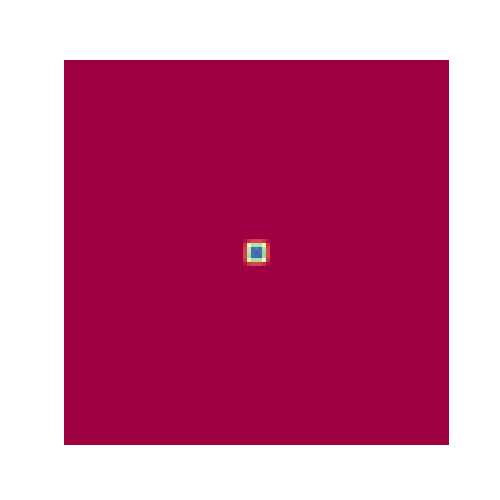
\includegraphics[width=.3\textwidth]{images/patch/1.png}}\hfill
            \subfloat[$t = 1000$]{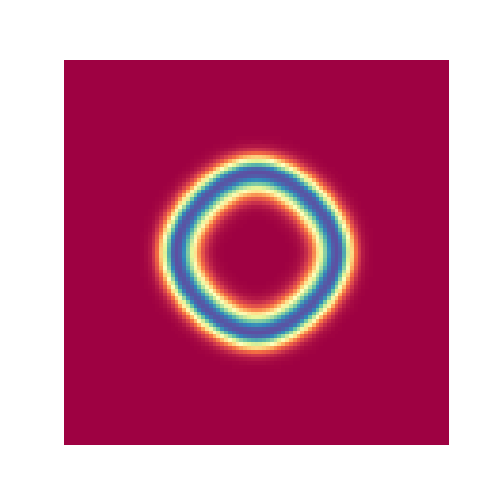
\includegraphics[width=.3\textwidth]{images/patch/2.png}}\hfill
            \subfloat[$t = 2000$]{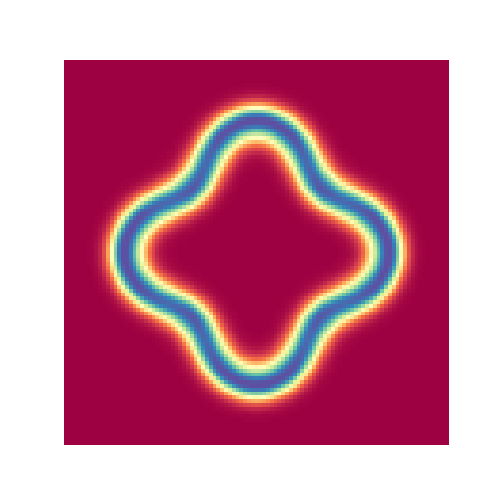
\includegraphics[width=.3\textwidth]{images/patch/3.png}}\hfill
            \subfloat[$t = 3000$]{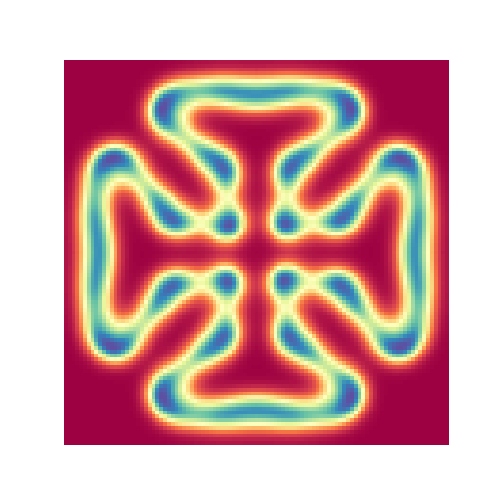
\includegraphics[width=.3\textwidth]{images/patch/4.png}}\hfill
            \subfloat[$t = 4000$]{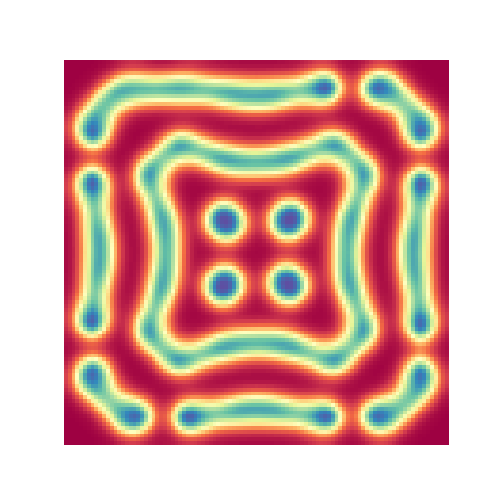
\includegraphics[width=.3\textwidth]{images/patch/5.png}}\hfill
            \subfloat[$t = 5000$]{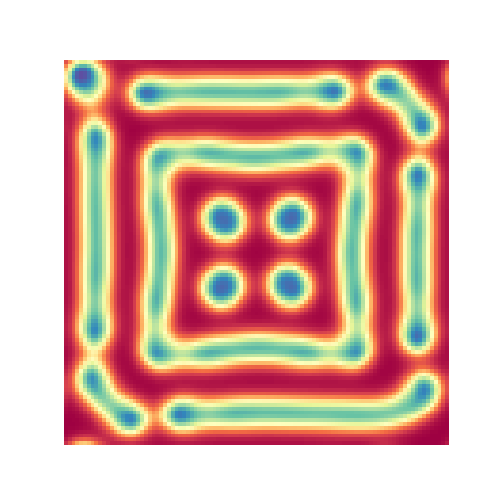
\includegraphics[width=.3\textwidth]{images/patch/6.png}}\hfill
            \caption{Gray-Scott simulation under \textit{patch} initialisation ($f = 0.03$, $k = 0.06$)}
\label{fig:patch}
\end{figure}

\begin{figure}[!h]
\centering
            \subfloat[$t = 0$]{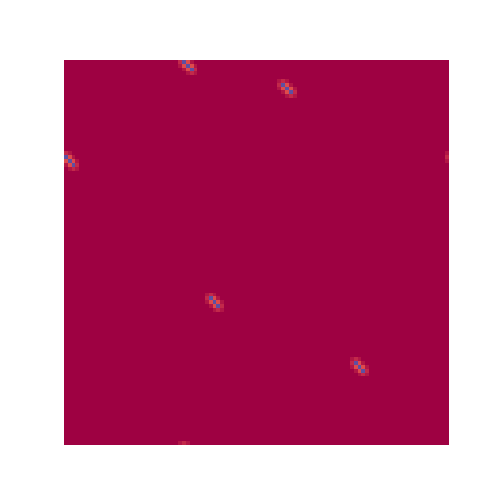
\includegraphics[width=.3\textwidth]{images/splatter/1.png}}\hfill
            \subfloat[$t = 200$]{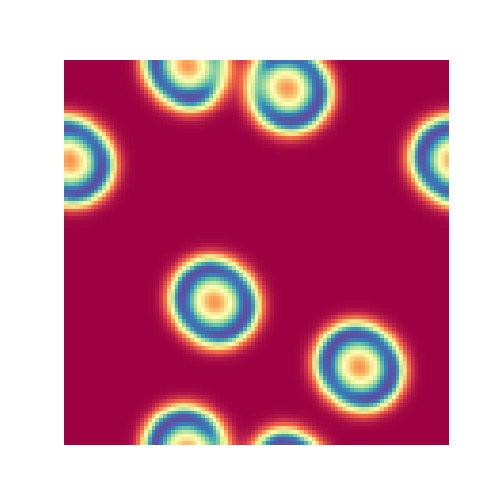
\includegraphics[width=.3\textwidth]{images/splatter/2.png}}\hfill
            \subfloat[$t = 500$]{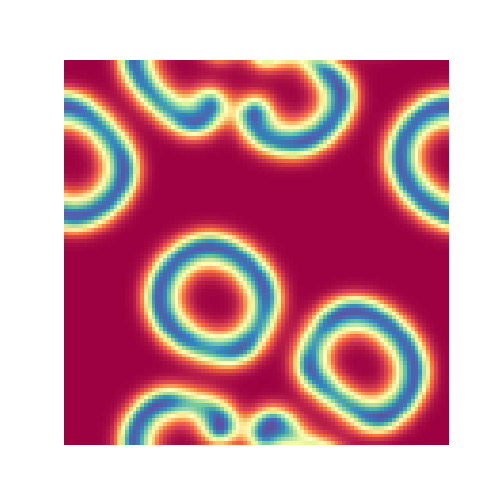
\includegraphics[width=.3\textwidth]{images/splatter/3.png}}\hfill
            \subfloat[$t = 1000$]{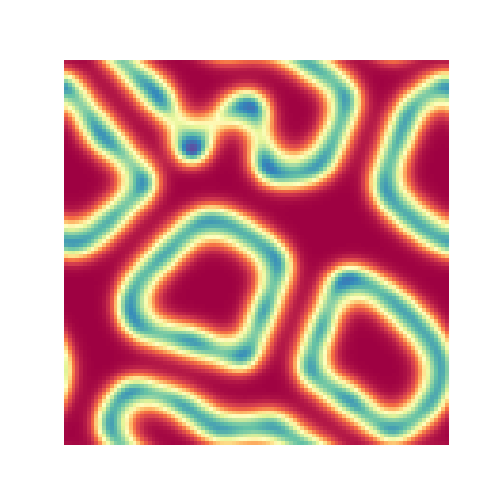
\includegraphics[width=.3\textwidth]{images/splatter/4.png}}\hfill
            \subfloat[$t = 2000$]{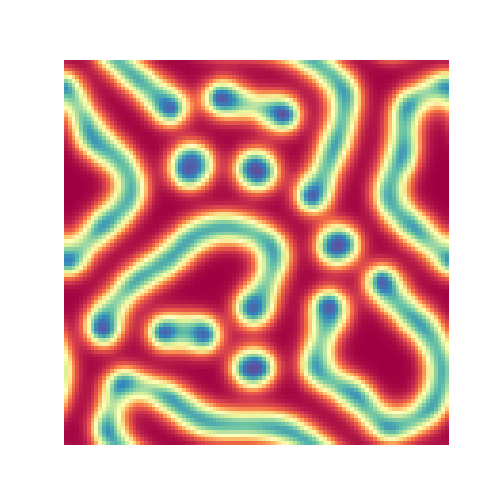
\includegraphics[width=.3\textwidth]{images/splatter/5.png}}\hfill
            \subfloat[$t = 5000$]{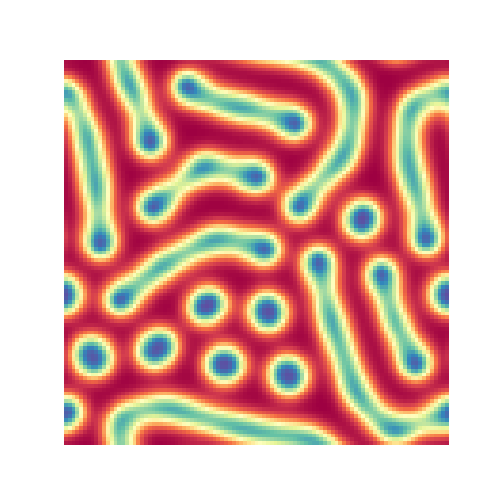
\includegraphics[width=.3\textwidth]{images/splatter/6.png}}\hfill
            \caption{Gray-Scott simulation under \textit{splatter} initialisation ($f = 0.03$, $k = 0.06$)}
\label{fig:splatter}
\end{figure}

\subsection{Chromosome}
The chromosome is made up of two vectors, \textit{state} and \textit{control}. The state vector contains the parameters of model, feed and kill rate, as two real numbers, $f$ and $k$. The control vector encodes the volatility of these parameters as real numbers $df$ and $dk$. The toolkit allows the user to initialise chromosomes in one of two ways. The first choice is to sample a random uniform distribution with $0.0 \leq f \leq 0.30$ and $0.0 \leq k \leq 0.08$. The boundaries are based on the nontrivial region depicted in Munafo's phase diagram in Figure~\ref{fig:xmorphia}. The second choice is to sample pairs close to the saddle-node bifurcation threshold $f = f(4+k)^2$ depicted as the solid line in Figure~\ref{fig:pearsons-threshold}. Values of $f$ is picked uniformly between the roots of the bifurcation parabola, $0.0$ and $0.25$. $k$ is the positive solution of this parabola $k = \frac{1}{2}\sqrt{f} - f$ perturbed by $\pm 10\%$ Gaussian noise and truncated at $k = 0$.

\subsection{Fitness and Selection}
Once the population of chromosomes has been initialised, we consider an objective function. As before, we simulate a true CA based on the goal parameters and maintain a surrogate cellular automata which is regularly synchronised with the true CA. The loss for a single cell is calculated by finding the difference in density between the true and surrogate cell as a fraction of the true density. The loss of the whole CA is the mean of these values and the fitness is defined as $1 - \textnormal{loss}$. This is a continuous extension of the XOR loss used for life-like CA. In roulette selection, each member of the population has a probability of progressing to the next generation equal to their fitness divided by the sum of the fitnesses of every individual in that population. In truncation selection, individuals are ranked by fitness and a fraction of the top ranking candidates are picked.\\

Selection comes in two flavours, \textit{plus} and \textit{comma}. Under plus-selection, parents and children alike are considered for progression to the next generation. This is the standard setting we used for life-like CA too. Under comma-selection, only offspring can progress to the next generation. We implement this setting as it enforces a "lifetime" of one generation on all candidates which promotes exploration outside of local optima. The downside to this is that it is easy for promising solutions to die out if they do not immediately pass on their advantageous characteristics to the next generation. This hinders convergence.\\

Crossover and mutation are dependent on the evolutionary algorithm being used. The two key evolutionary algorithms implemented are an evolutionary strategy and a genetic algorithm. We explore these in turn.

\subsection{Evolutionary Strategy}
Evolutionary strategies (ES) are black-box optimization algorithms suited to continuous domains. Some ES use fitness-based recombination where parents with a higher fitness produce more offspring[CITE]. In this case, selection pressure and exploitation of generational knowledge are pursued simultaneously, so traditional environmental selection can be omitted. For our use case, we stick with a fitness-independent recombination method and a separate environmental selection scheme to allow more flexibility in tuning both processes.\\

An ES individual has the form $a_i: (\bm{x}, \bm{\sigma}, F(\bm{x}))$ which are the state parameters, control parameters, and fitness respectively. The control parameters define the average size of mutation and are specific to each individual. ES also often use more than 2 parents for recombination unlike GA. Typically, all children are produced from the top $\rho$ parents with $\rho \leq \mu$. Common recombination operators include:
\begin{itemize}
  \item Discrete: For each of the offspring's state variables, one of the $\rho$ parents is picked from which to inherit.
  \item Intermediate: The offspring's state is the mean of the states of the parents.
  \item Weighted Intermediate: The offspring's state is a weighted combination of the parent states with a weighting function that increases monotonically with fitness.
\end{itemize}

A fundamental idea in ES is parameter control by self-adaptation. For a self-adapting ES, control parameters are evolved just like state parameters. Each of the $\lambda$ offspring are generated as follows
\[b_i \gets
\begin{cases}
    \bm{x}_i = \bar{\bm{x}} + \bm{\sigma}_i\bm{N_i(0, I)},\\
    \bm{\sigma_i} = \bar{\bm{\sigma}}e^{\tau\bm{N_i(0, I)}},\\
    F_i = F(\bm{x}_i)
\end{cases}
\]
Where we define the intermediate recombination operator as the arithmetic mean
\[
  \bar{\bm{y}} = \frac{1}{\rho}\sum_{m=1}^{\rho}{\bm{y}_m}
\]
where $\bm{y}_m$ is the $\bm{y}$ property of the $m^{th}$ best mixing parent by fitness. The state vectors receive Gaussian mutation with variance defined by the control parameters and the control parameters receive log-normal mutation with variance dependent on a constant learning rate $\tau$. This is usually set proportional to $\frac{1}{\sqrt{n}}$ but can be tuned as a hyperparameter. The terms $\bm{N_i(0, I)}$ are normally distributed vectors with the same dimensions as the vector being mutated.\\

We implement this strategy but, in the style of Hansen et al.\cite{hansen2015evolution}, we apply mutation in two parts. There is a common mutation applied to all control parameter components of $\tau_1{N_i(0, 1)}$ and a specific mutation applied to each component individually of $\tau_2\bm{N_i(0, I)}$ with $\tau_1 = n^{-\frac{1}{2}}$ and $\tau_1 = n^{-\frac{1}{4}}$.\\

% \begin{figure}[!h]
% \centering  
%             \hfill
%             \subfloat[Isotropic Mutation]{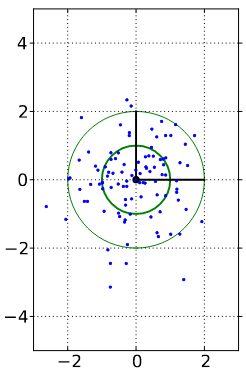
\includegraphics[width=.2\textwidth]{images/es-iso-mutation.png}}\hfill
%             \subfloat[Axis Parallel Mutation]{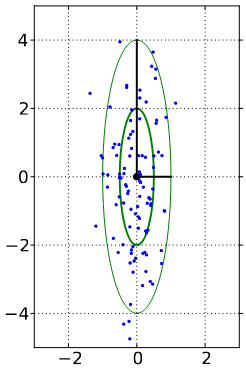
\includegraphics[width=.2\textwidth]{images/es-axis-parallel-mutation.png}}\hfill
%             \subfloat[General Mutation]{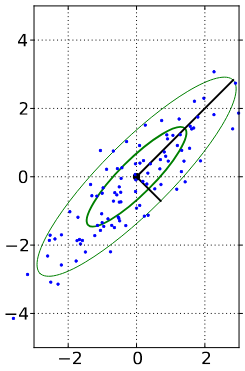
\includegraphics[width=.2\textwidth]{images/es-general-mutation.png}}\hfill\hfill
%             \caption{}
% \label{fig:es-mutations}
% \end{figure}

% However, the self-adapting ES uses isotropic mutations or axis parallel mutations which means it is difficult to choose appropriately sized mutations for correlated state variables. To address this, we use a covariance matrix adaptation evolutionary strategy (CMA-ES) which is the state-of-the-art in continuous domain evolutionary strategies. \\

% TODO?

\subsection{Genetic Algorithm}
The genetic algorithm performs crossover, recombination, mutation, and selection as usual. The crossover method used is a combination of uniform crossover and blended crossover (BLX-$\alpha$). Uniform crossover is used on the state property of each chromosome. For two parents $x$ and $y$, a property of a child $c$ is defined by a value sampled uniformly from the interval between the corresponding property in the parents.
\begin{align*}
  c_f &\sim \mathit{Uniform}(\min(x_f, y_f),\ \max(x_f, y_f))\\
  c_k &\sim \mathit{Uniform}(\min(x_k, y_k),\ \max(x_k, y_k))
\end{align*}
However, the control property is different due to the BLX-$\alpha$ algorithm which combines exploration and exploitation. A traditional crossover algorithm seeks to exploit generational knowledge to create novel candidate solutions by deriving a child state interior to the boundaries defined by the parents' states. For example, consider a single-point crossover on a binary string. If both parents have a 1 in the $i^{th}$ position bit, it is impossible for the child to have a 0 in the $i^{th}$ bit. In this sense, BLX-$\alpha$ is not pure crossover as it explores areas of the search outside the parent-defined borders.

\begin{definition}[Blended Crossover (BLX-$\alpha$)]
We define the blended crossover of real numbers $x_i$, $y_i \in [a_i, b_i]$ with $x_i < y_i$ and parameter $\alpha \in \mathbb{R^+}$ as a sample\\
\[
  BLX(x_i, y_i, \alpha) \sim \mathit{Uniform}(x_i - \alpha(y_i - x_i),\  y_i + \alpha(y_i - x_i))
\]
\end{definition}
The hyperparameter $\alpha$ defines how much exploration the operator undertakes as a fraction of the difference between the parent states. In the special case $\alpha = 0$ this is another uniform crossover and when $\alpha$ is maximised, this approaches a uniform mutation operator where the value of a child gene is a uniform sample across the predefined gene boundaries $a_i$ and $b_i$.\\

\begin{figure}[!h]
\centering
    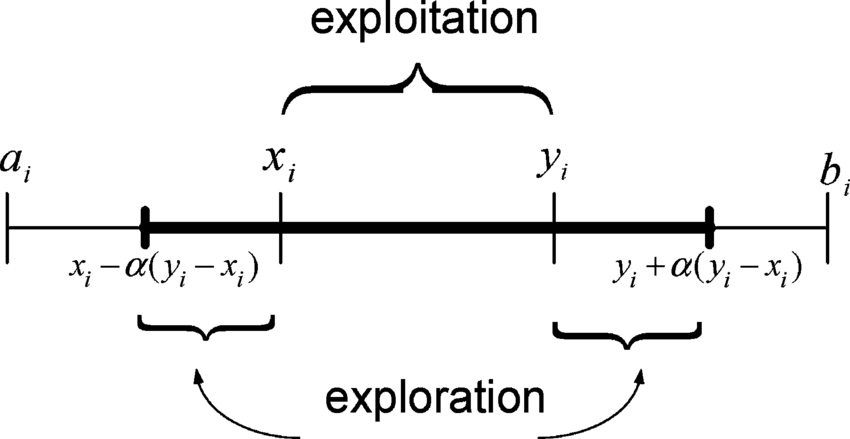
\includegraphics[width=.5\textwidth]{images/blx.png}
    \caption{Blended Crossover \cite{abido2006multiobjective}}
\label{fig:blx-alpha}
\end{figure}

To ensure exploration is occurring for state properties too, shrink mutation is applied. This is where Gaussian noise is added to $f$ and $k$. The variance of this noise is dictated by the control property 


\section{Software Engineering Design}
